\documentclass[a4paper,10pt]{article}
\usepackage[utf8x]{inputenc}
\usepackage{float}
\usepackage{graphicx}
\usepackage{placeins}
\usepackage{natbib}

%opening
\title{}
\author{}

\begin{document}

\maketitle

\begin{abstract}

\end{abstract}
%%
\section{Background}
%
It has been known for some time that convectively generated gravity waves feed back on the
organisation of tropical convection \citep{wheeler1999convectively}. Remote momentum and temperature
changes in the troposphere, communicated through the propagation of convectively generated gravity
waves, condition the troposphere for further convection triggering or suppression
\citep{bretherton1989gravity}. The role of gravity waves in the convection adjustment process
was further investigated by Mapes \citep{mapes1993gregarious}, who details the ``gregarious'' nature
of mesoscale tropical convection due to the evolution of gravity bores, which displace low-level
parcels upward. 

The work of Nicholls quantitively details the importance of mode 1 and 2 gravity waves in adjusting
the neighbouring cloud-free environment. Using a 2D CRM, Lane and Reeder (ref) later showed that
indeed a mode 3 gravity waves plays a large role in modifying CIN in the neighbourhood of
convection. 

Shutts and Gray use a numerical model investigate the role of Coriolis. 
Shutts and Gray examined the role of gravity waves in adjusting the environment of isolated clouds
in highly rotating frames. 

How gravity waves propagate into the stratosphere is well documented.
\citep{alexander1995gravity} show how high freq gravity waves in stratosphere above a storm show
good correlation between vertical wavelengths of gravity waves and depth of convective heating.

However, despite a number of idealised studies, questions remain about the role of gravity
waves in the troposphere. 

In an attempt to leave no stone unturned in constructing a complete picture, we revist the theory
of forced gravity waves in the hope of attaining quantitive understanding in previously
neglecting aspects to the problem. Using a linear, 2D, Boussinesq atmosphere, which is forced with
a sensibly prescribed heating term, we find an analytic solutions for vertical velocity, $w$, and
potential temperature, $b$. The effect of Coriolis are reserved for a subsequent paper. We apply a
similar technique to \citep{nicholls1991thermally}, who investigates the qualtitive upward flux of
energy in a system with a high rigid lid. Having an analytic solution allows us to cut computing
cost, and raise the lid into a regime where we have a purely radiating solution (i.e. the group
speed of the gravity waves is not large enough to rebound off the lid within our time domain). We
use this toy model to address the following questions:
\begin{itemize}
 \item What are the sensitivities to the horizontal lengthscale of heating in the far field
response?
 \item What are the consequences of a transient heat source? 
\end{itemize}
This paper directly addresses such questions, mainly through the inspection and quantification of
difference plots between selected configurations of our toy model. Section 2 will detail the
mathematics of our solution. Section 3 includes results from simulations probing the effect of
horizontal lengthscale, and transient effects of heating respectively. Section 4 contains a
summary and discussion. 

\pagebreak
%%
\section{Results}
Throughout this results section, we present model data for the vertical velocity, $w$,  and
potential temperature, $b$ fields, since both are influential in the organisation convection. Any
region with positive $w$, and high $b$ is likely to trigger convection, with the opposite likely to
suppress triggering.

\subsection{The Effect of Raising the Position of the Rigid Lid Upper Boundary Condition}
Figure ( \ref{raise_lid_t1} ) depicts the effect of increasing the
altitude of the upper lid. We observe the distribution of energy increases aloft, indicating a
radiative effect. Quantitative insights into the upward flux of energy may be obtained from this
data. For example, it appears that as the lid height increases the vertical flow at the top of plot
windows becomes more uniform.

\begin{figure}[h!]
  \caption{}
  \centering
    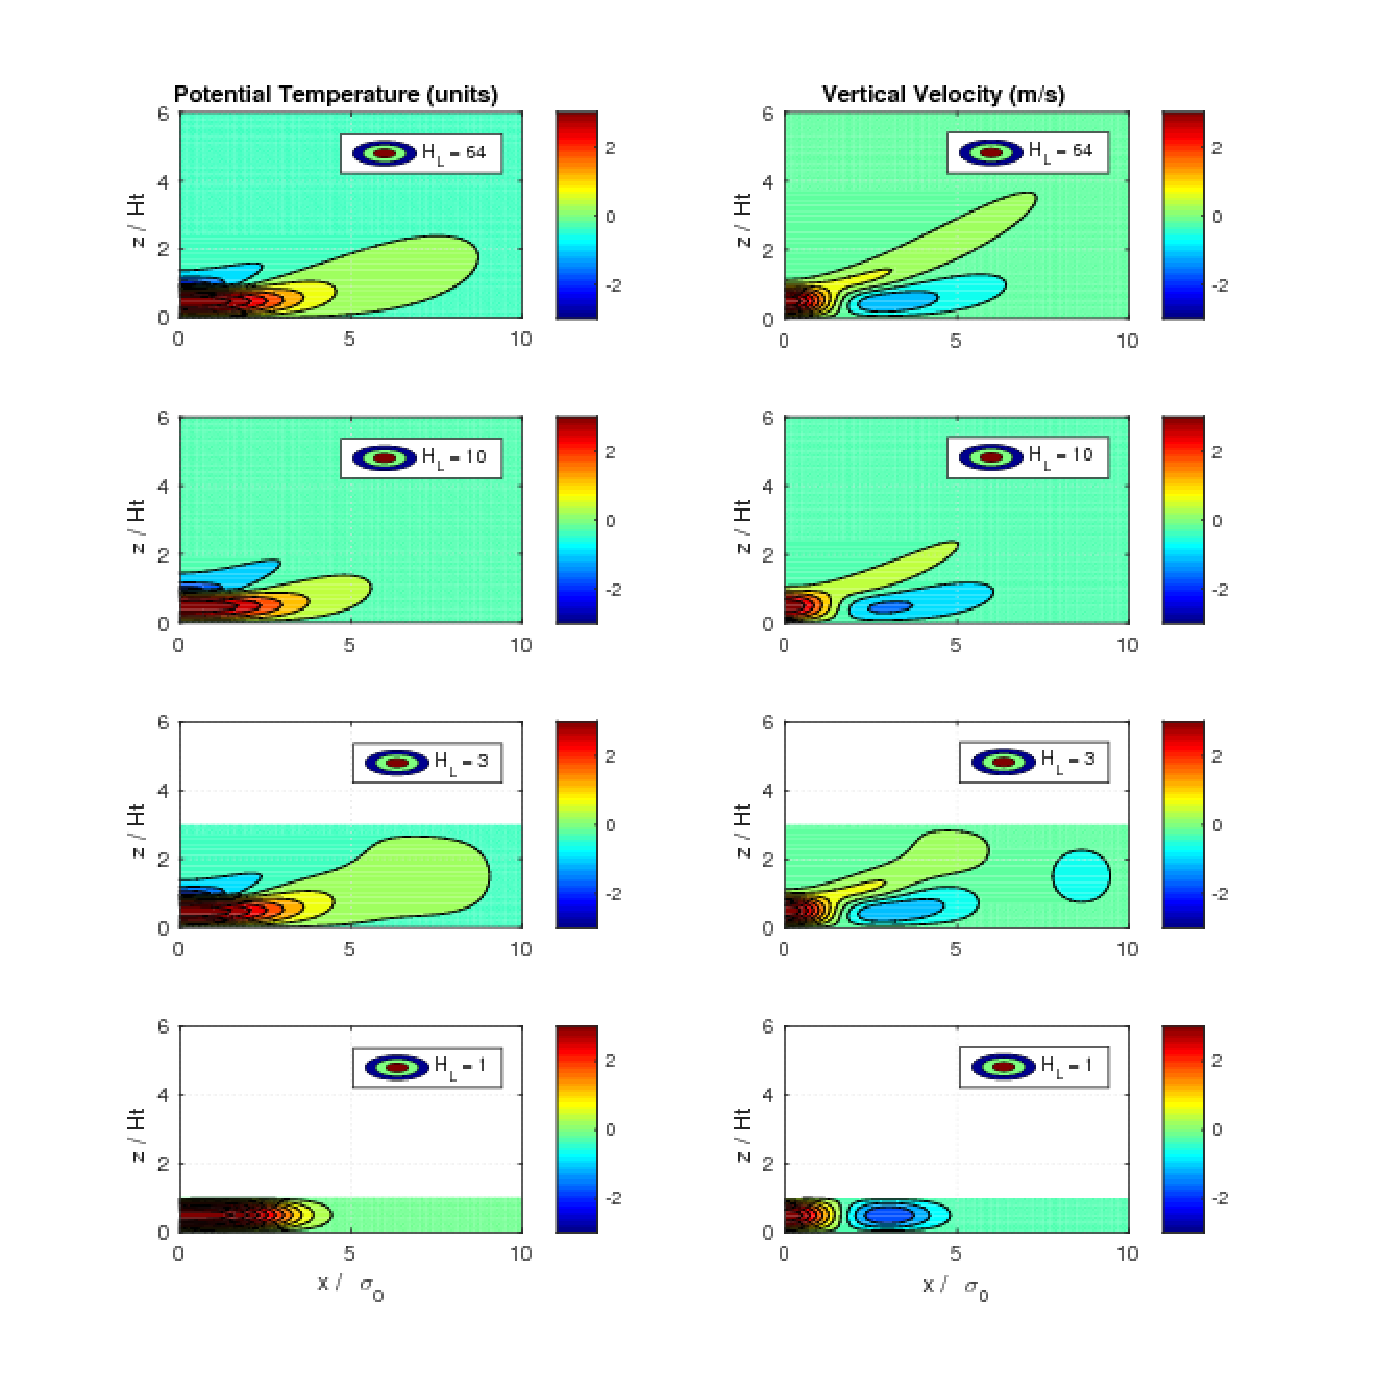
\includegraphics[width=1\textwidth]{raise_lid_t1.pdf}
  \label{raise_lid_t1}
\end{figure}

\begin{figure}[h!]
  \caption{}
  \centering
    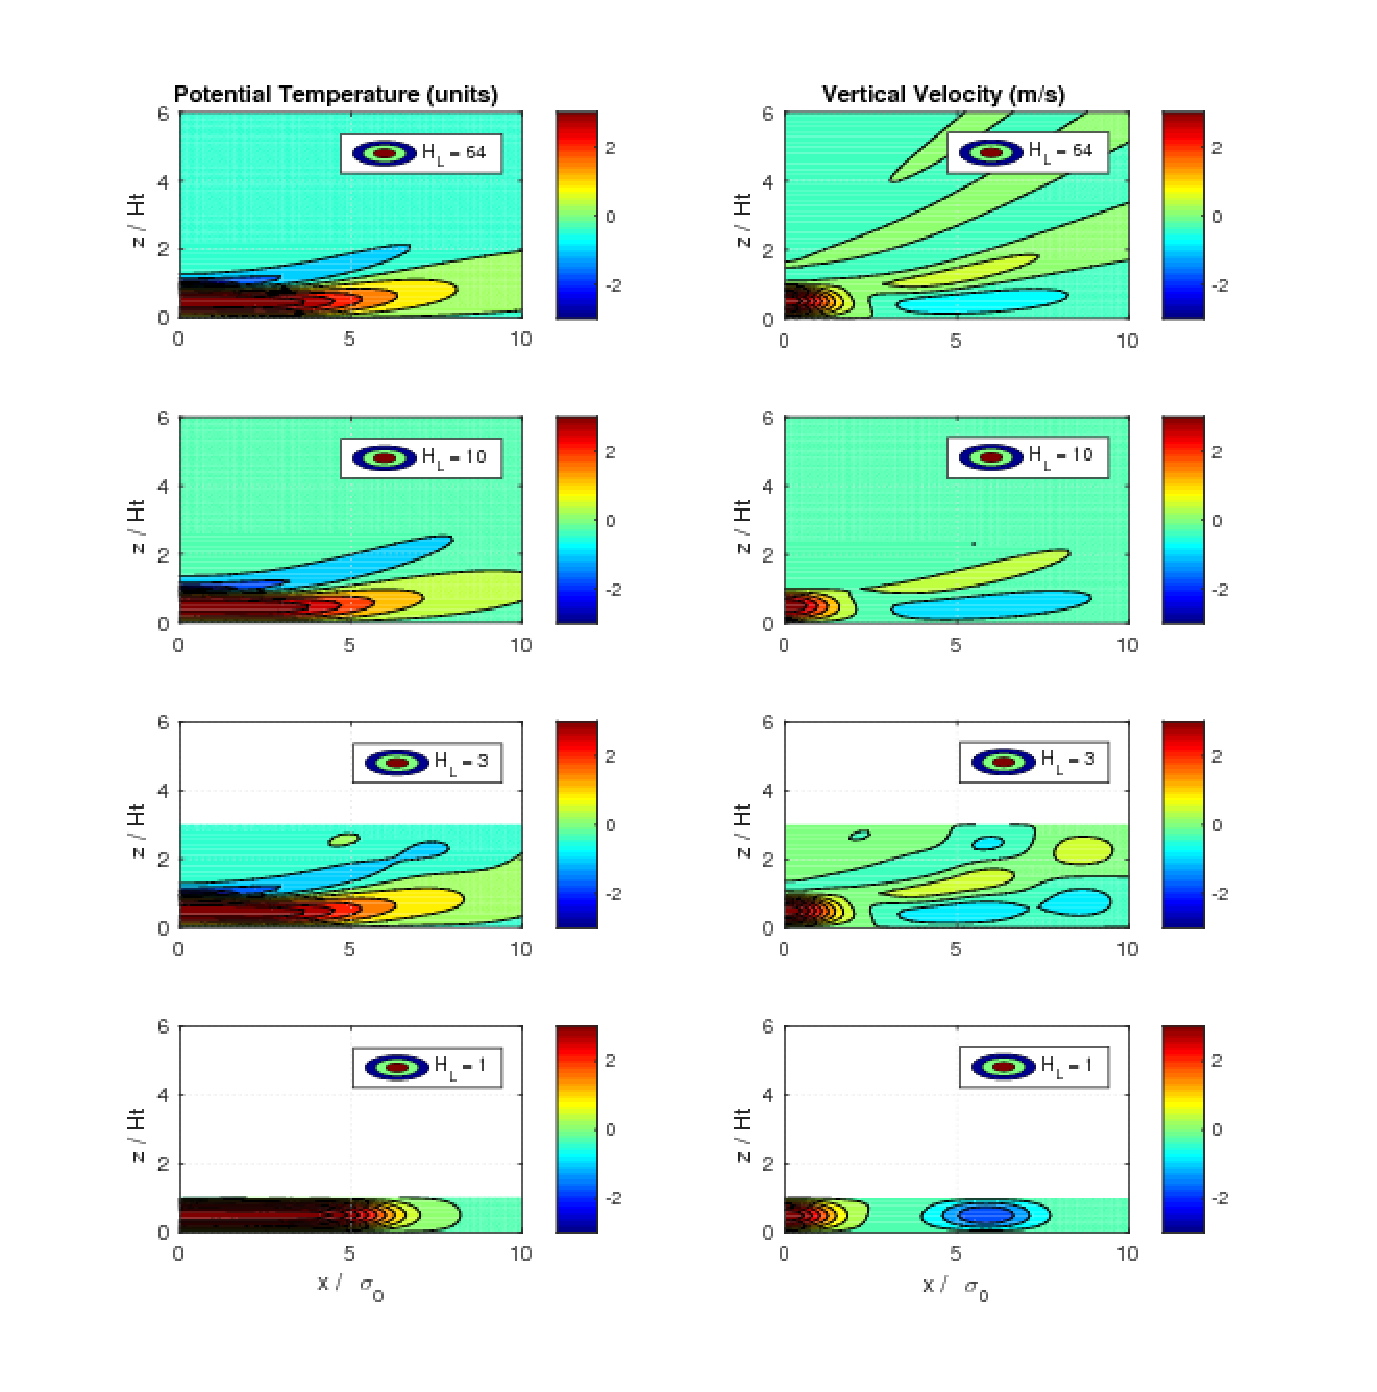
\includegraphics[width=1\textwidth]{raise_lid_t2.pdf}
  \label{raise_lid_t2}
\end{figure}

%\Floatbarrier

Along with figure (  \ref{raise_lid_t2} ) we note the horizontal evolution of the w-response, which
is characterised by modes with phase speed $\frac{N H}{j \pi}$ (recall $j$ is the vertical
harmonic number) is qualitatively unaffected by the process of raising the lid. The vertical
structure however varies considerably more between $H_L = 1$ and  $H_L = 3$ than it does between
$H_L = 10$ and $H_L = 64$ which is indicative of convergence of the $w$ and $b$ solution (at least
in the troposphere). We also note that as the height of the lid increases the influences of
the heating excite a deeper mode, characterised by a larger horizontal phase speed, as
expected. The confining effect of the lid intensifies subsidence in the troposphere, meaning
neighbouring convection is unlikely to be triggered. However, continuity considerations suggest
enhanced triggered elsewhere. In the present case, we
observe the only candidate region for this amplified ascent would be the heated region. We note that
the horizontal suppression of convection is more locally intense, but less mobile, in the trapped
cases.

One can better understand the time evolution of the system through figure HERE
%(\ref{Hovmoller_steady.eps})

\subsection{Transient Heating}
Assigning the time dependence of the heating function to be a simple boxcar function (on/off), we
investigate the influence of a transient heat source. Figure
(\ref{vertical_cross_transient}) shows the $w$ and $b$ response
field to such transient heating which is switched off at a time $t = 30mins$ (a reasonably
realistic convection timescale, note). Advancing down the panels, we evolve at a time step of 15
minutes.

\begin{figure}[h!]
  \caption{}
  \centering
    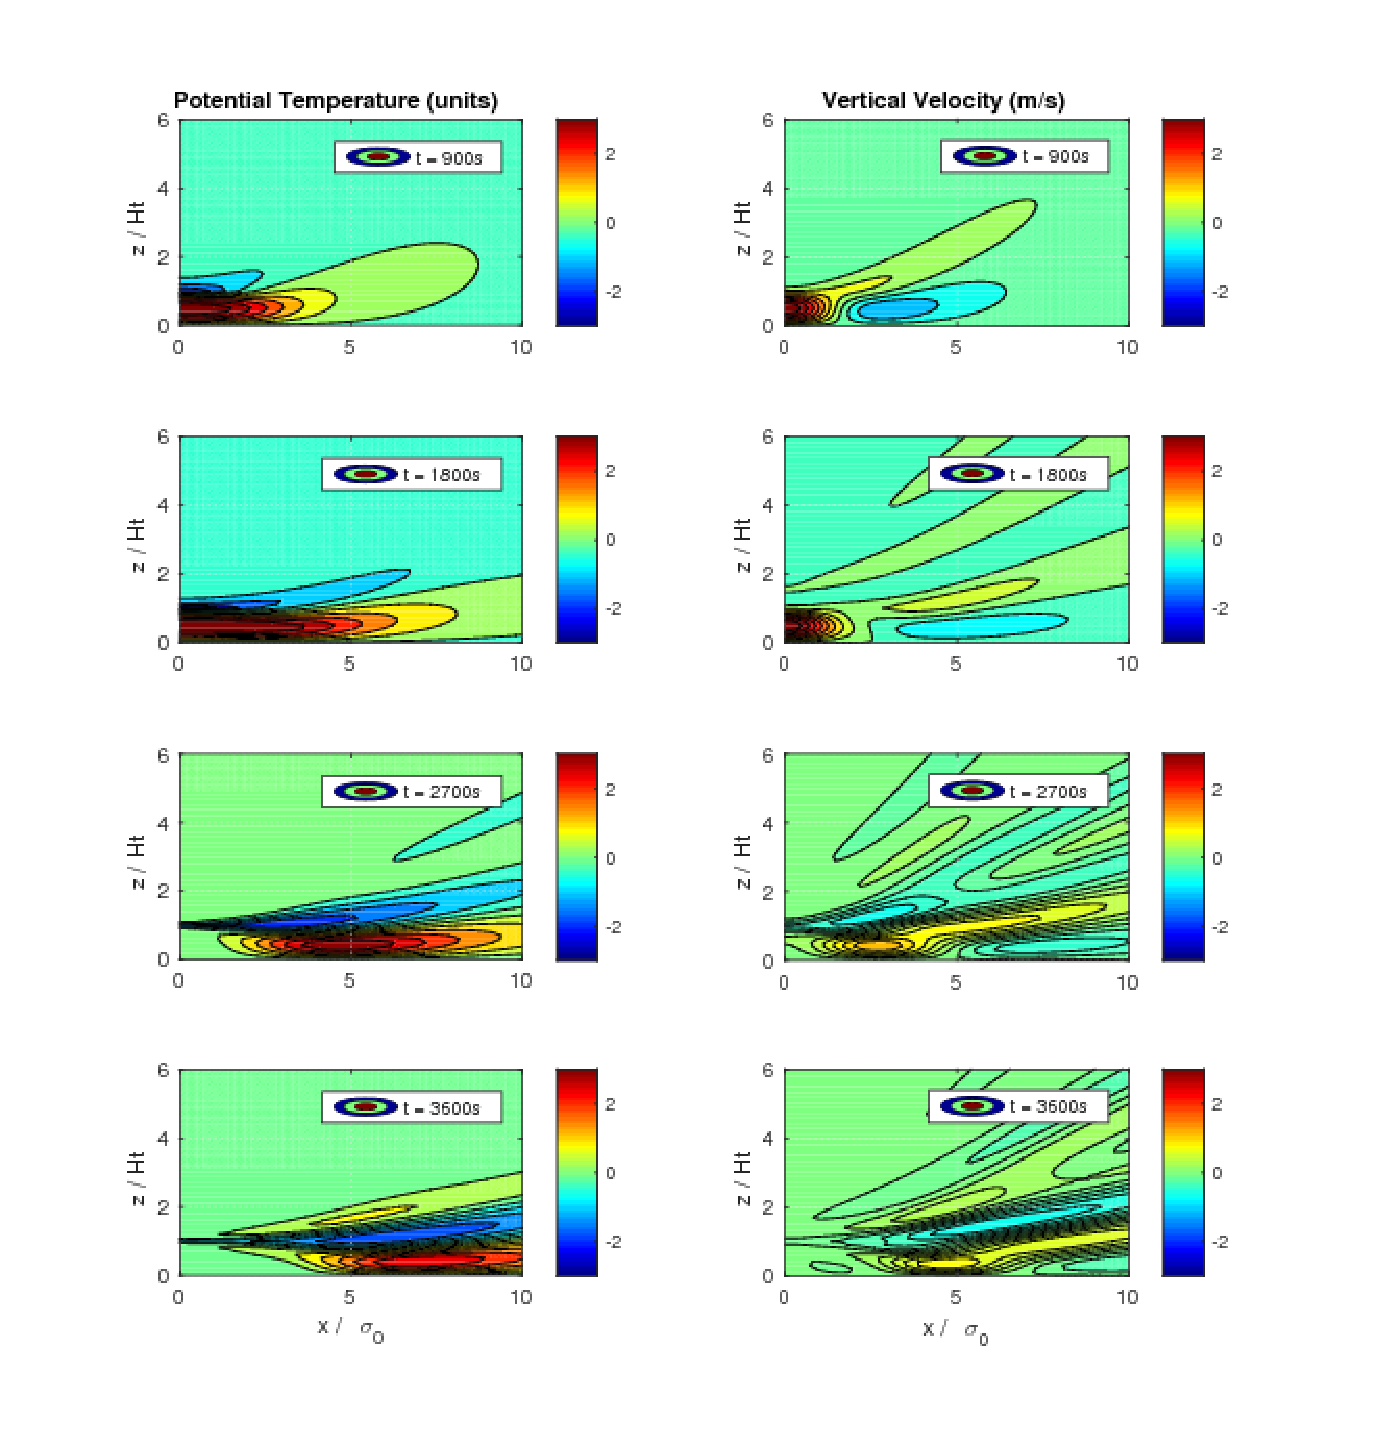
\includegraphics[width=1\textwidth]{Transient_vertical_cross.pdf}
  \label{vertical_cross_transient}
\end{figure}

%\Floatbarrier

The most notable effect of truncating heating is the occurrence a propagating region of ascent in
the troposphere (as seen in figure (\ref{Hovmoller_transient_diffs})), which is absent in all
the steady heating cases considered previously. 
\begin{figure}[h!]
  \caption{}
  \centering
    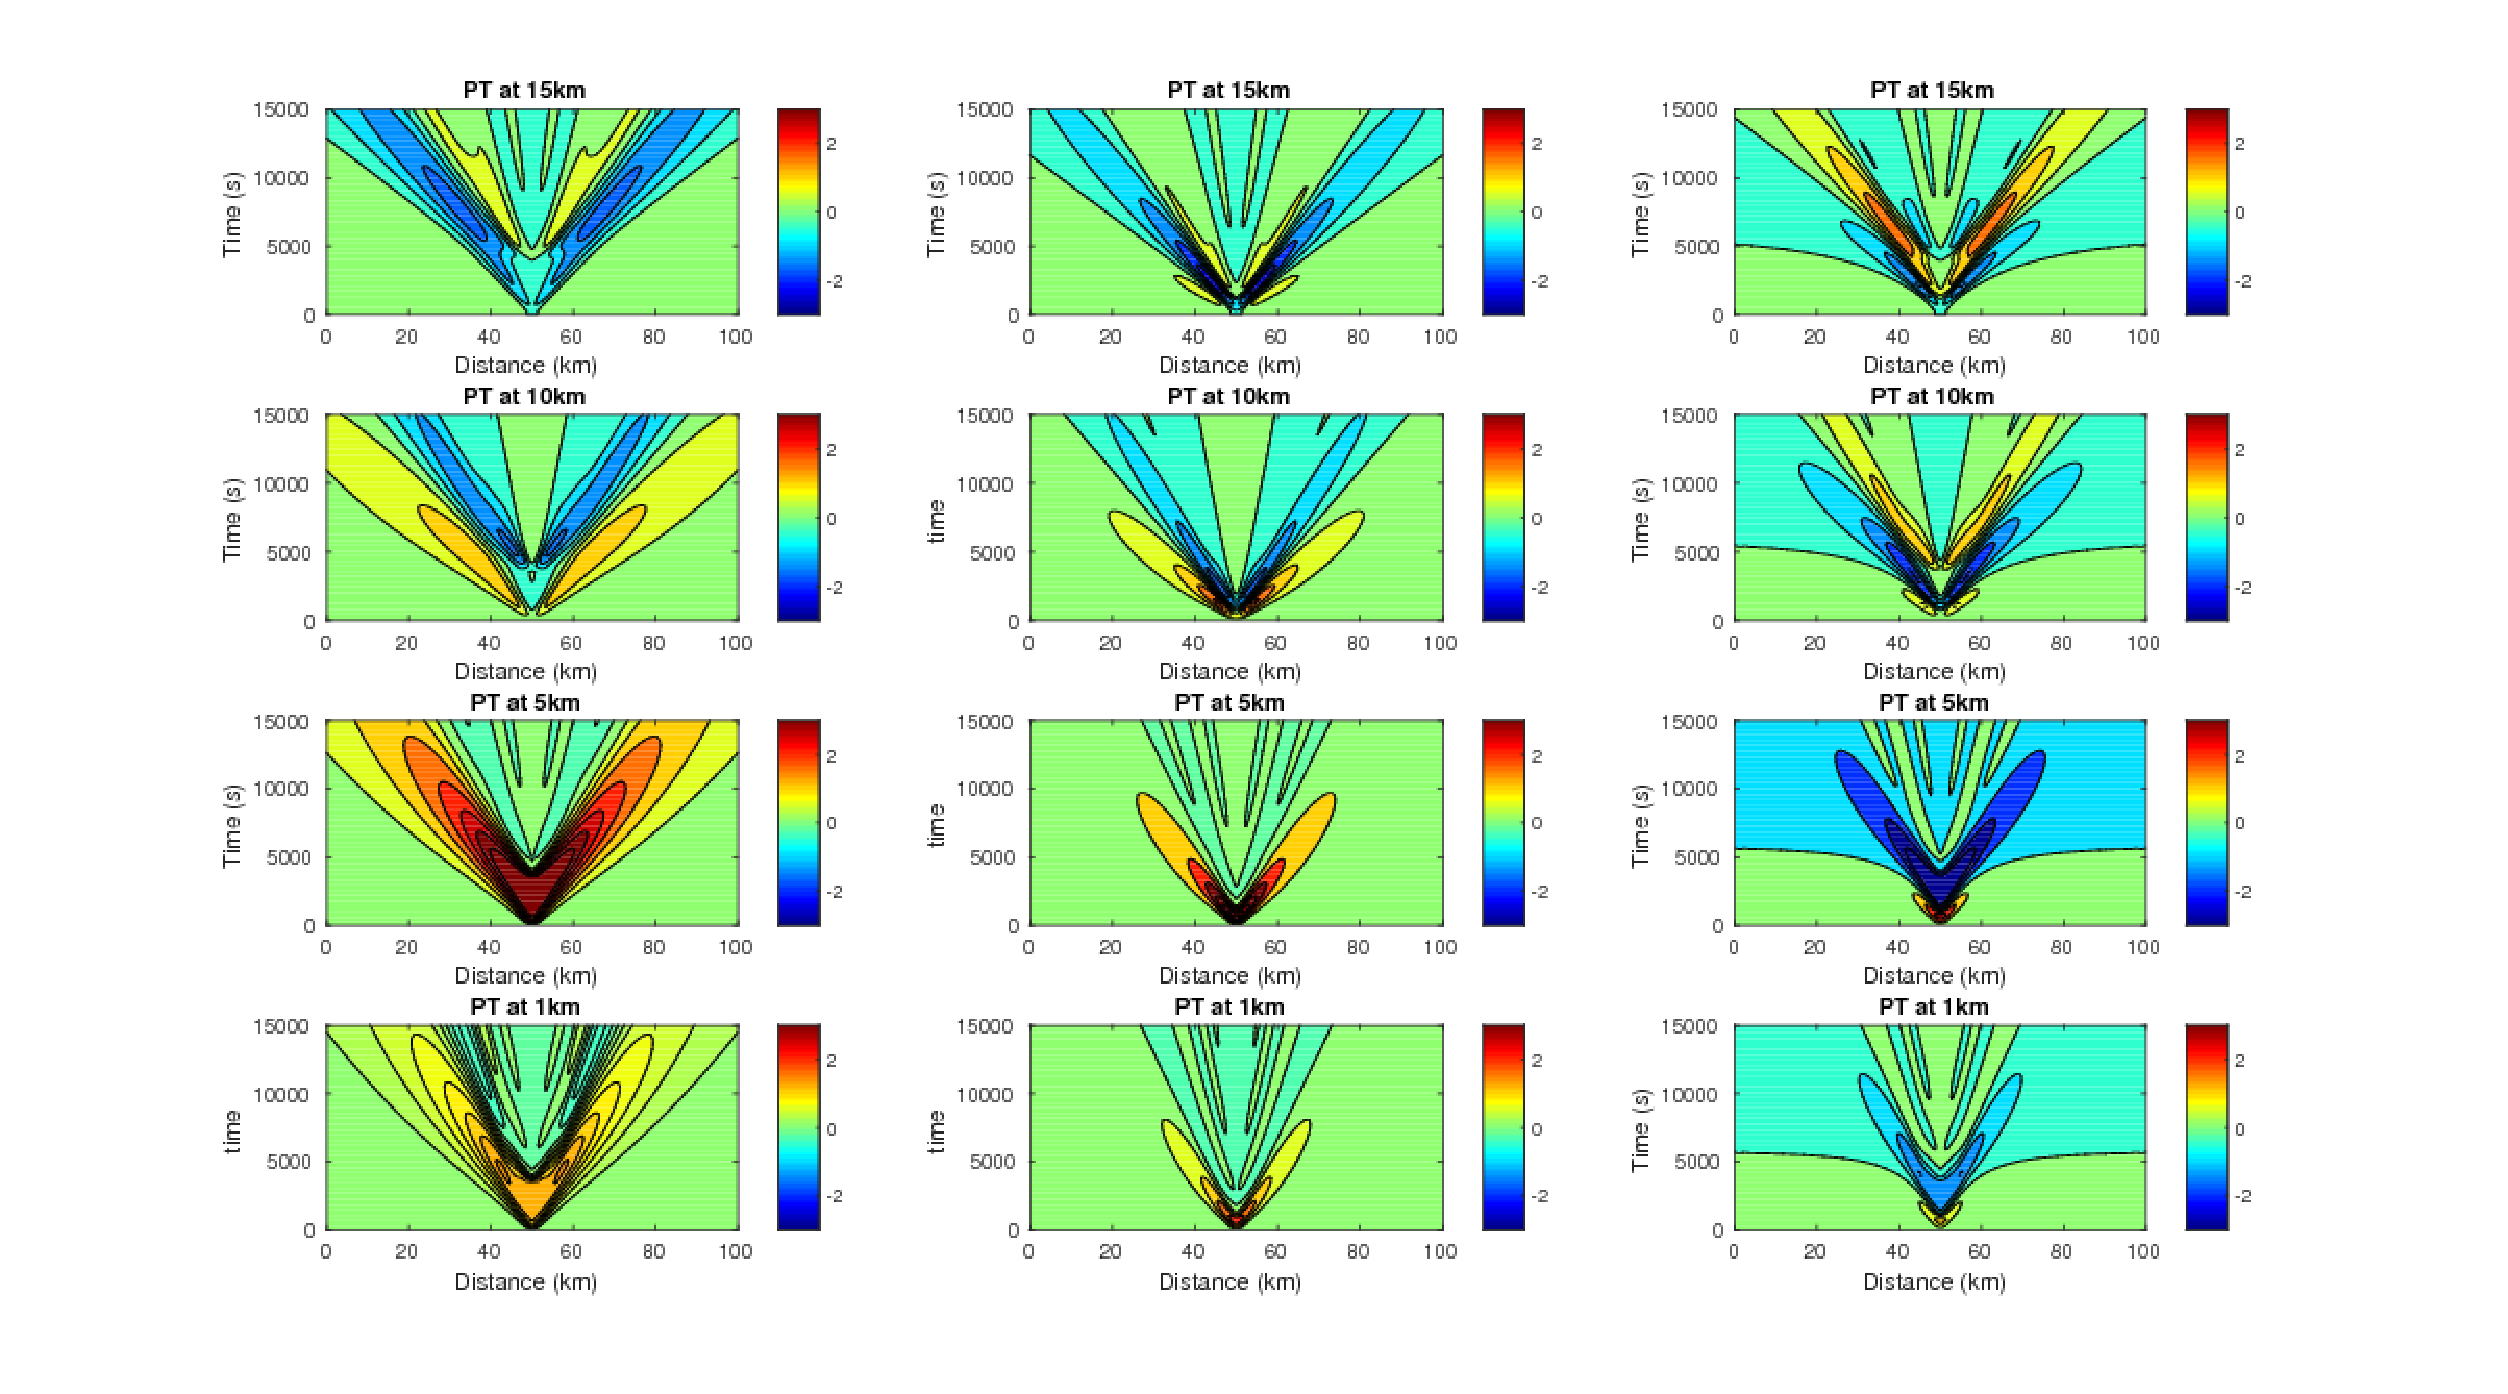
\includegraphics[width=1\textwidth]{hovmoller_transient_diffs.pdf}
  \label{Hovmoller_transient_diffs}
\end{figure}

%\Floatbarrier


HERE The reader is directed to the top right hand panel of
figure (2.4), in the region of $x = 2$. Counterintuitively, this bservation appears to suggest that
terminating heating could trigger a weak convective event in the neighbourhood.


\subsection{TO INCLUDE}
\begin{figure}[h!]
  \caption{}
  \centering
    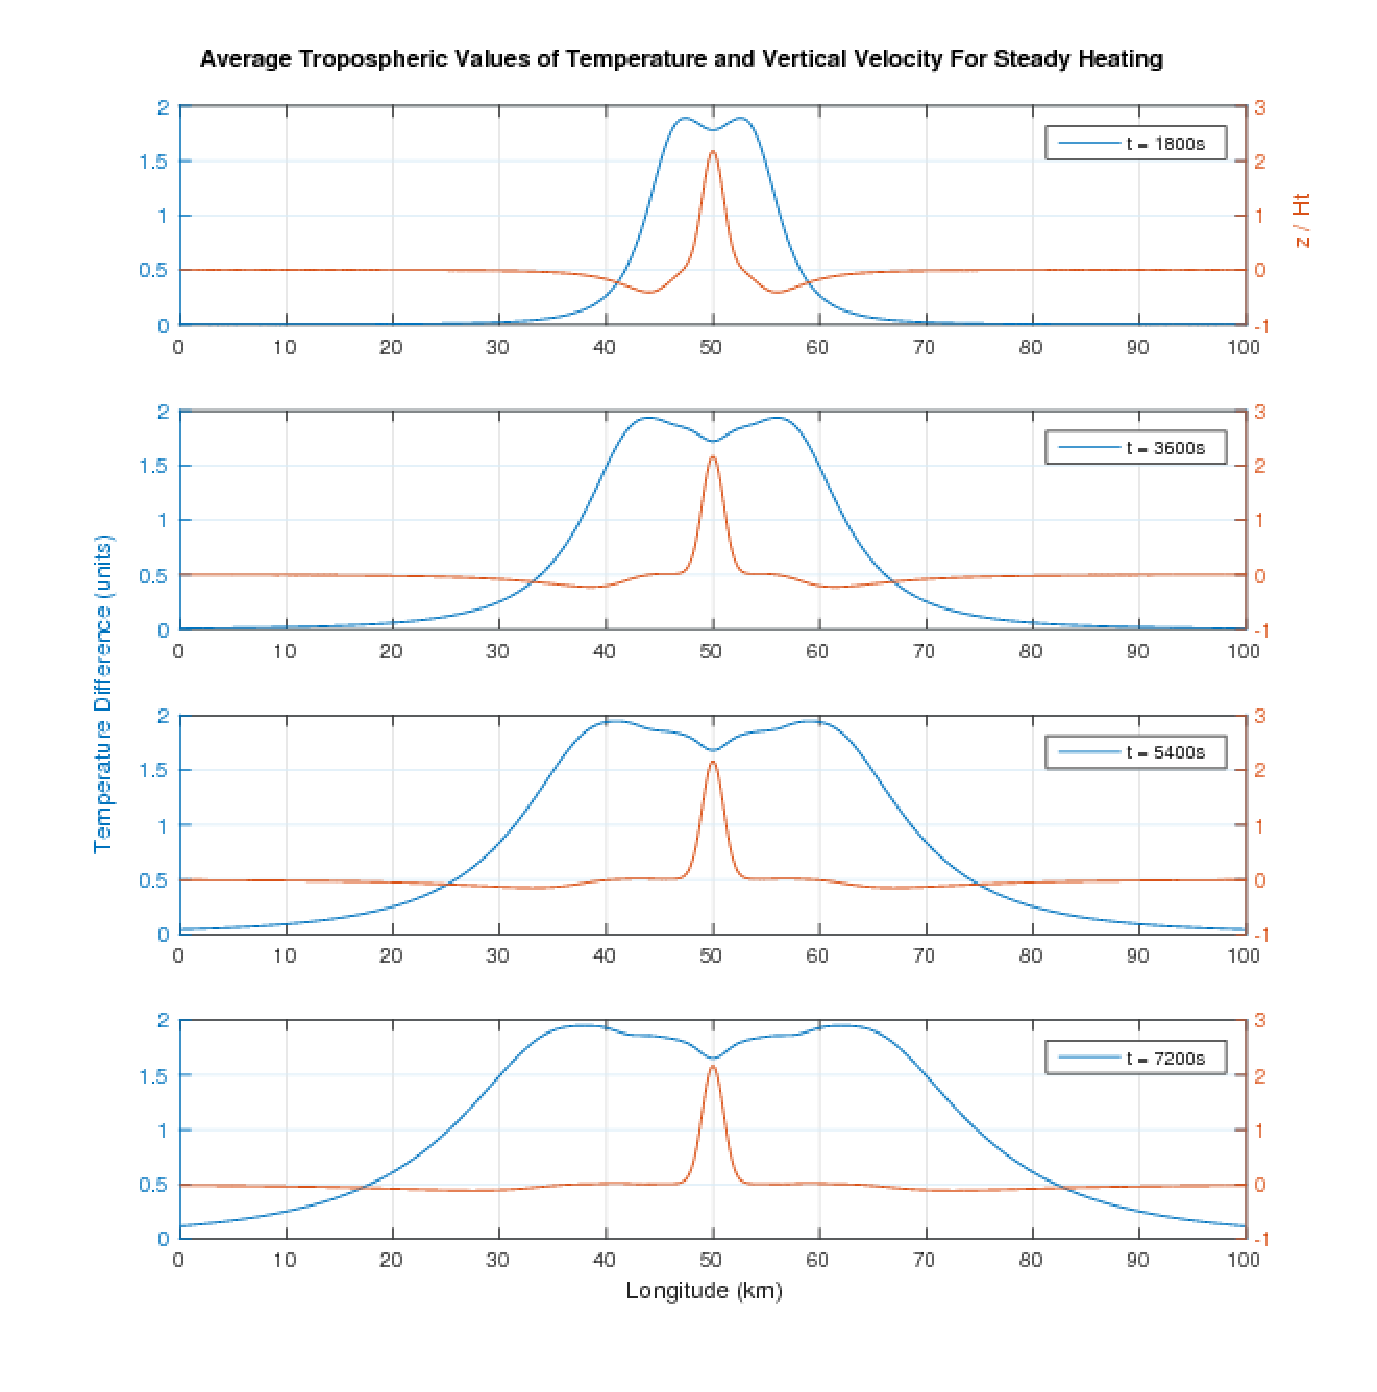
\includegraphics[width=1\textwidth]{trop_values_steady.pdf}
  \label{trop_values_steady}
\end{figure}

\begin{figure}[h!]
  \caption{}
  \centering
    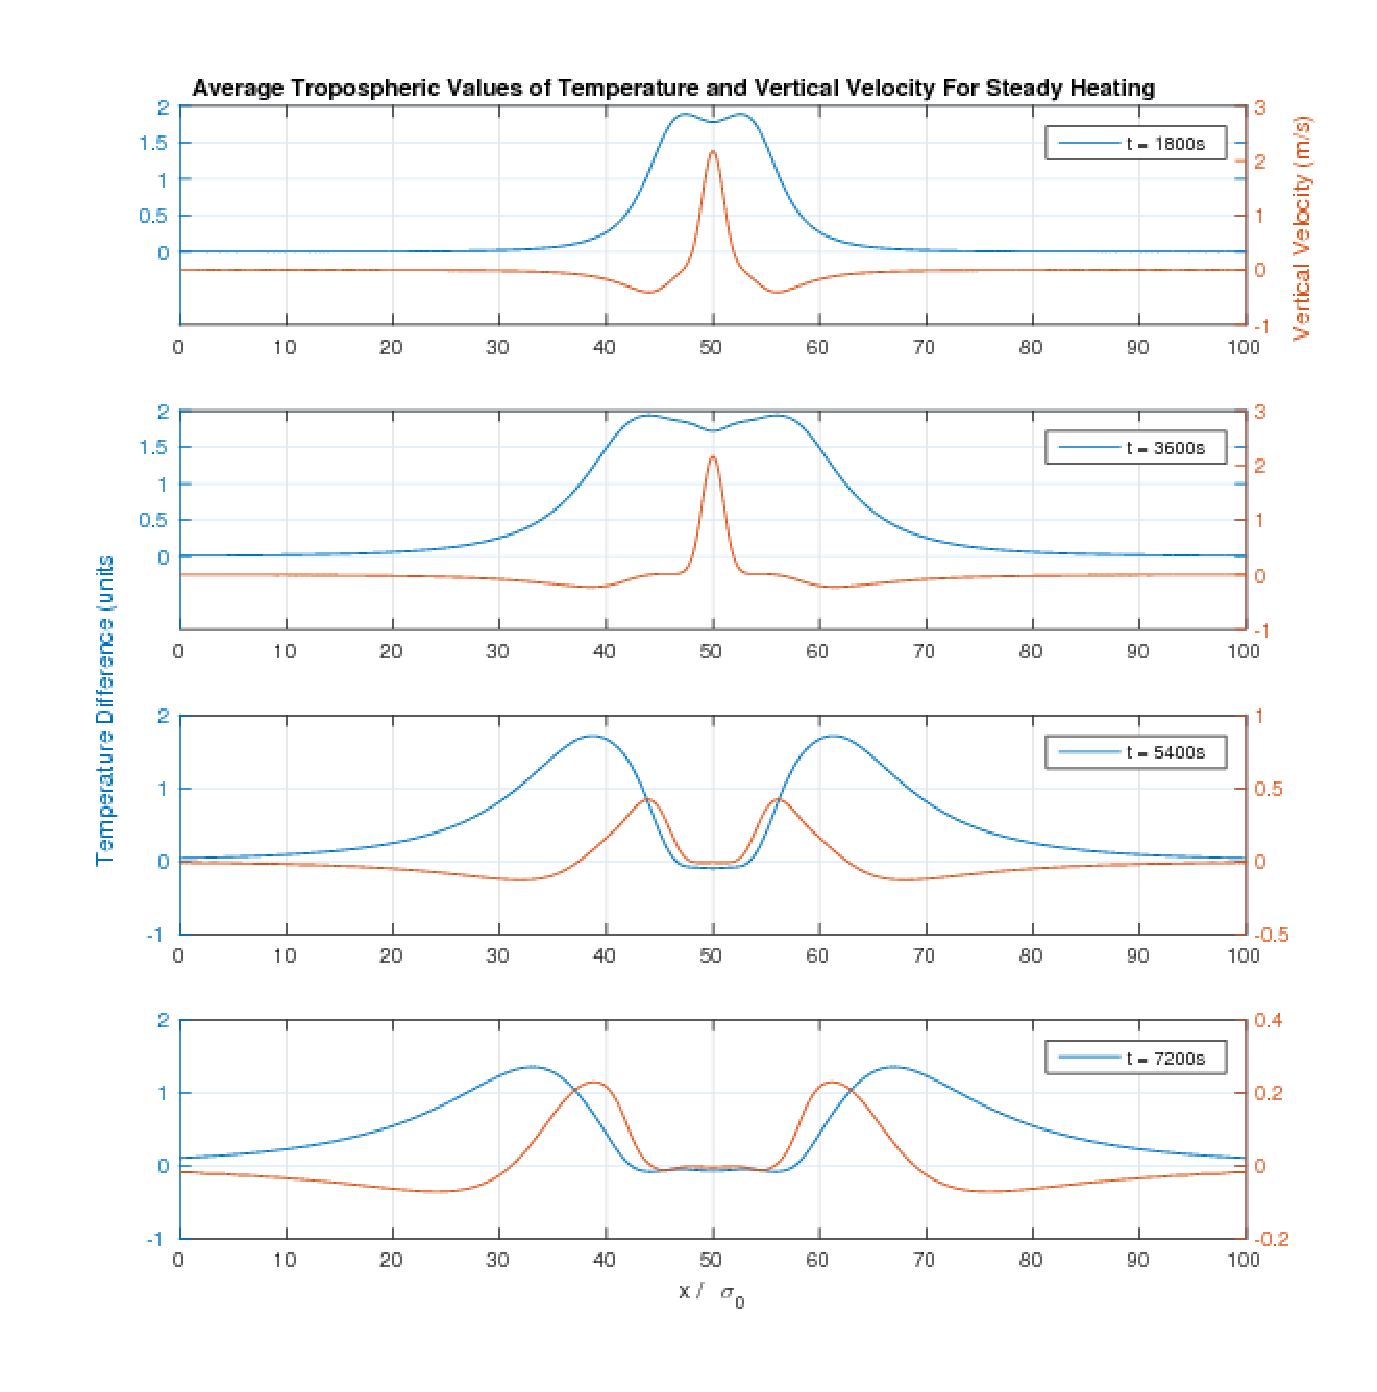
\includegraphics[width=1\textwidth]{trop_values_transient.pdf}
  \label{trop_values_transient}
\end{figure}

\begin{figure}[h!]
  \caption{}
  \centering
    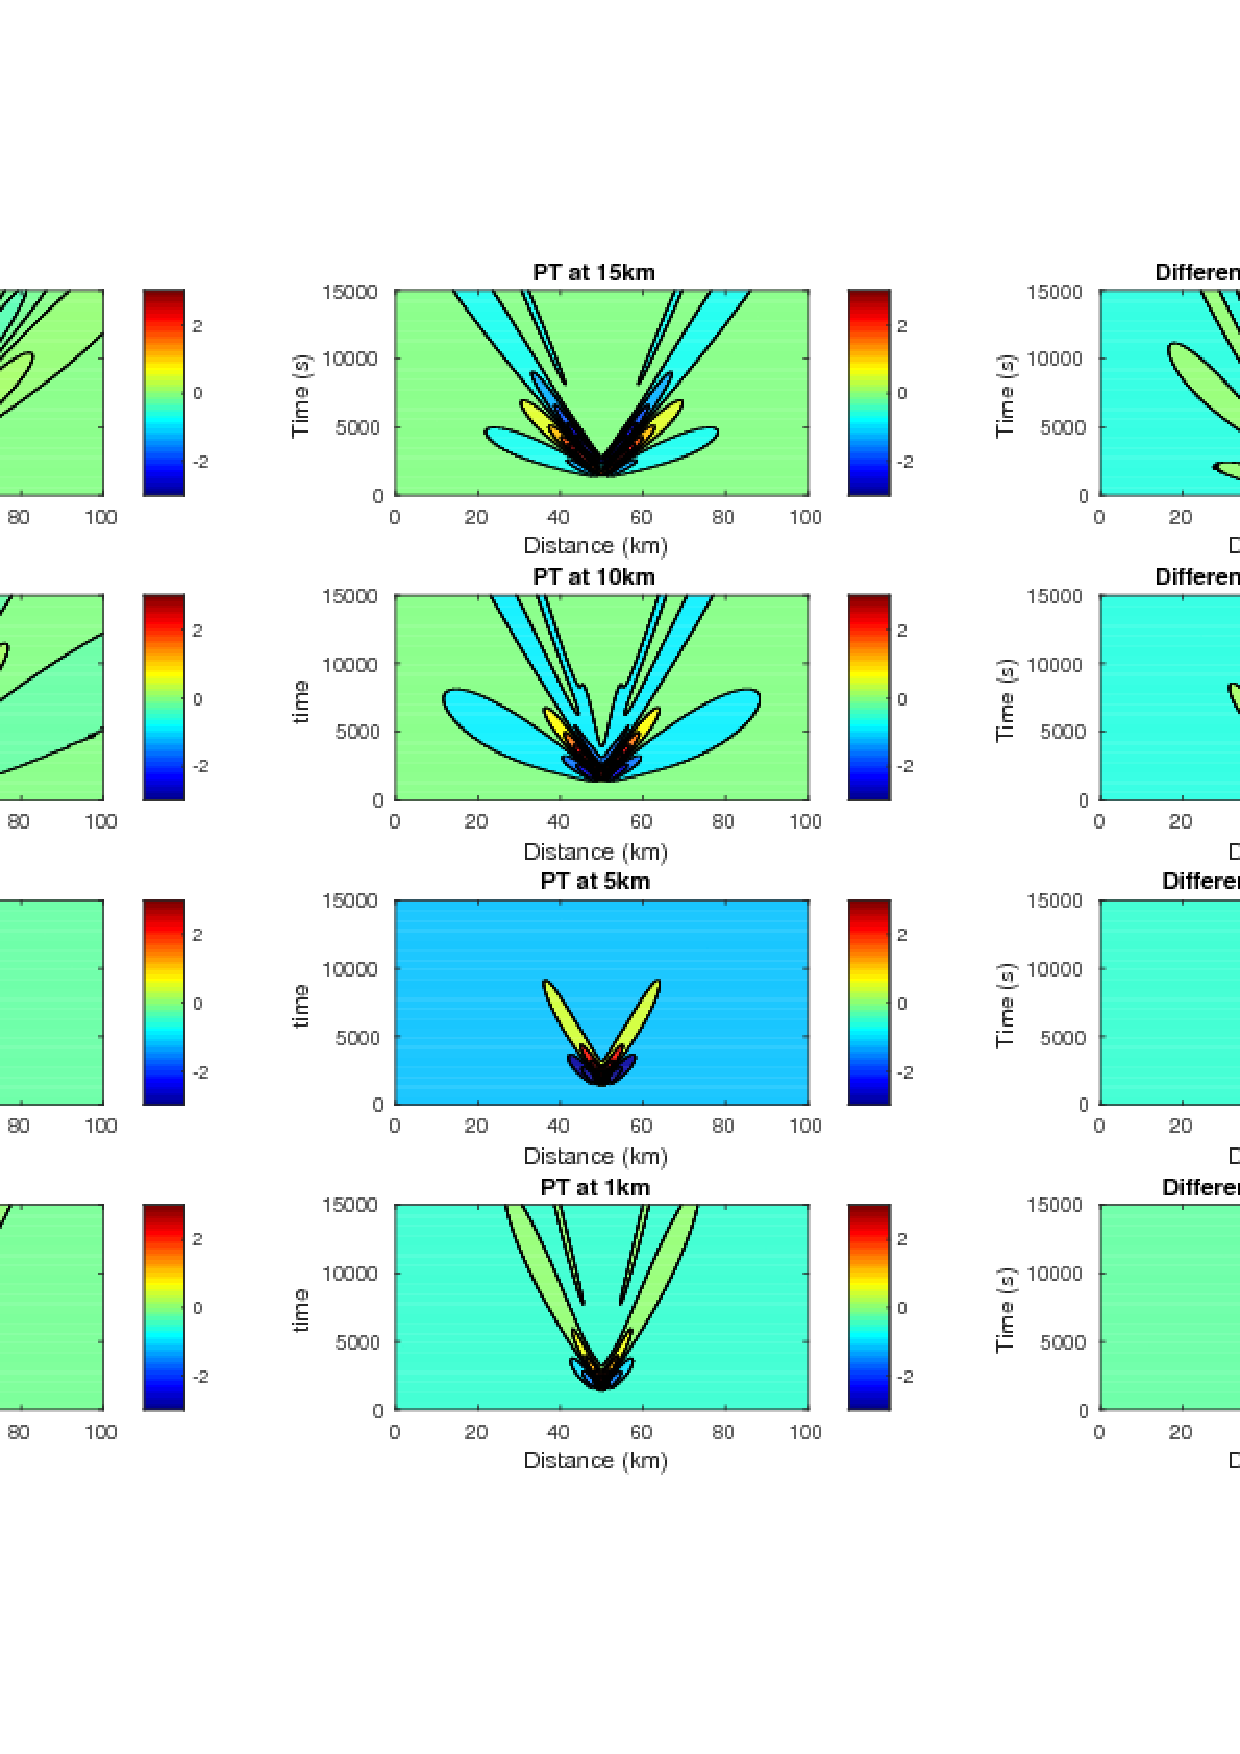
\includegraphics[width=1\textwidth]{hovmoller_transient_diffs_w1.pdf}
  \label{trop_values_transient_diff_w1}
\end{figure}

\begin{figure}[h!]
  \caption{}
  \centering
    \includegraphics[width=1\textwidth]{hovmoller_transient_diffs4.pdf}
  \label{trop_values_transient_diff_w1}
\end{figure}


\begin{figure}[h!]
  \caption{}
  \centering
    \includegraphics[width=1\textwidth]{hovmoller_b_steady.pdf}
  \label{hovmoller_b_steady}
\end{figure}


\bibliographystyle{acm}
\bibliography{paper1.bib}

\end{document}
